\chapter{R7acuity: An Independent Ideal-Observer Monte Carlo Model}
\label{ch:r7acuity}

\section{Why a second, structurally independent model}

Chapter~\ref{ch:acuity_models}'s closed-form predictors failed clinical validation
(Chapter~\ref{ch:validation}). That failure alone cannot distinguish between two
explanations: a genuine problem with the specific frequency-cutoff formula, or a
data-scarcity problem (the clinical dataset has only $n=5$ points and one
non-monotonic outlier). R7acuity is a Monte Carlo template-matching ideal-observer
simulation (Watson \& Ahumada, 2008) --- a structurally different architecture, built
specifically to provide a second, independent test that shares the same validated
optics but nothing else with the closed-form route.

\section{The psychometric threshold procedure}

For a 4-alternative-forced-choice tumbling-E task, the simulated observer's proportion
correct at optotype size (MAR, arcmin) $m$ is fit to a logistic psychometric function
in log-MAR space:
\begin{equation}
p(m) = 0.25 + \frac{0.75}{1+\exp\big(-\beta(\log_{10}m - \log_{10}m_t)\big)}
\end{equation}
where the fitted threshold parameter $m_t$ directly gives the threshold MAR at the
criterion $p=0.625$ (halfway between chance $0.25$ and ceiling $1.0$) by construction
--- no separate root-finding is needed. The threshold optotype size \emph{is} the MAR
directly (this model's own $5\times5$-unit optotype convention exactly matches the
clinical MAR definition), so $\text{logMAR}=\log_{10}(m_t)$ needs no cutoff-frequency
conversion, unlike the MTF-based routes of Chapter~\ref{ch:acuity_models}.

\section{Noise-sigma calibration}

The model's one free parameter --- additive Gaussian noise $\sigma$ on the neural image
--- is calibrated \emph{once}, against a single non-clinical reference condition
(diffraction-limited, emmetropic, $3\mm$ aperture, target $1.0$ arcmin MAR / $20/20$),
by log-space bisection, \textbf{before} the model is ever run against any clinical
dataset, and is never re-tuned afterward regardless of validation outcome.

\section{Closed-form cross-check}

Independent of the Monte Carlo procedure, two closed-form approximations (specified,
not derived, per the governing brief) reuse this project's already-validated
Strehl/VSOTF machinery directly:
\begin{equation}
\text{logMAR}_{Strehl} = 25\log_{10}(S), \qquad
\text{logMAR}_{VSOTF} = \frac{50}{3}\log_{10}(\text{VSOTF})
\end{equation}
computed by running the exact ASM pipeline \emph{twice} per point (once for the actual
condition, once for its diffraction-limited reference) --- this cross-check is
``closed-form'' only in how it combines Strehl/VSOTF into a logMAR number, not in how
it obtains those two inputs, which require full wave-optics propagation each time.

\begin{figure}[htbp]
\centering
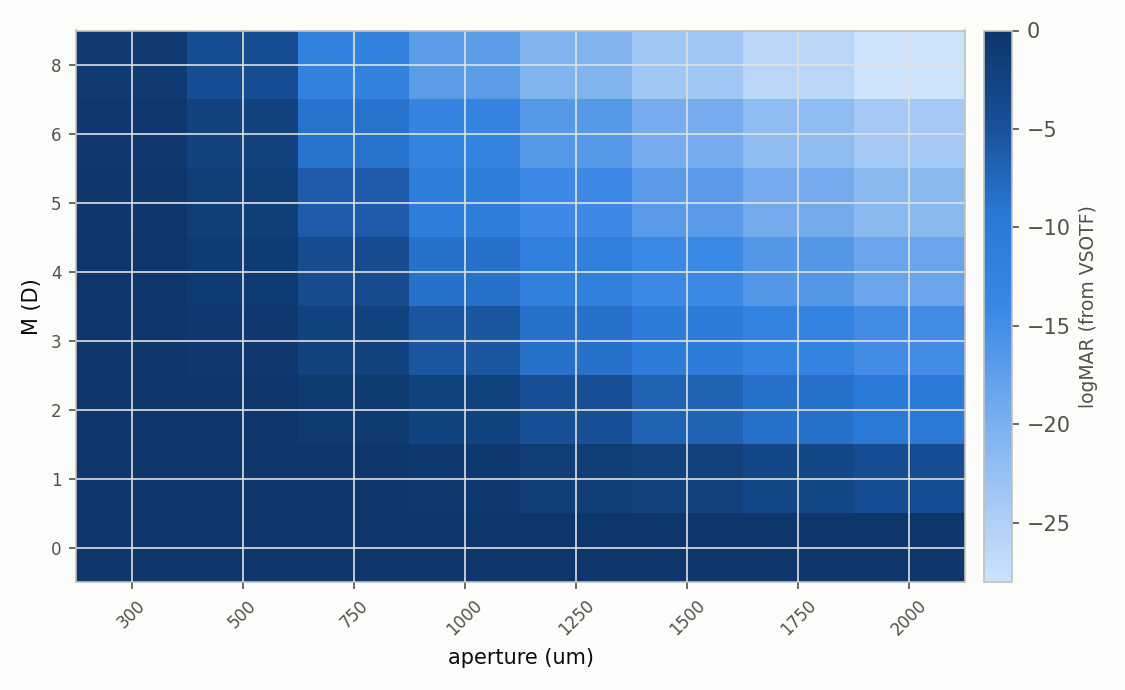
\includegraphics[width=0.85\textwidth]{figures/fig_r7acuity_closedform_heatmap.png}
\caption{R7acuity closed-form cross-check: predicted logMAR (from VSOTF) across a representative aperture $\times$ myopia grid.}
\label{fig:r7-closedform}
\end{figure}

{\small
\begin{longtable}{rrrrrr}
\caption{R7acuity closed-form Strehl/VSOTF cross-check, full sweep.}\label{tab:r7-full}\\
\toprule
a\_hole (um) & M (D) & Strehl & VSOTF & logMAR (Strehl) & logMAR (VSOTF) \\
\midrule
\endfirsthead
\multicolumn{6}{c}{\tablename\ \thetable\ -- continued}\\
\toprule
a\_hole (um) & M (D) & Strehl & VSOTF & logMAR (Strehl) & logMAR (VSOTF) \\
\midrule
\endhead
\bottomrule
\endfoot
300.000 & 0.000 & 1.000 & 1.000 & 0.000 & 0.000 \\
500.000 & 0.000 & 1.000 & 1.000 & 0.000 & 0.000 \\
750.000 & 0.000 & 1.000 & 1.000 & 0.000 & 0.000 \\
1000.000 & 0.000 & 1.000 & 1.000 & 0.000 & 0.000 \\
1250.000 & 0.000 & 1.000 & 1.000 & 0.000 & 0.000 \\
1500.000 & 0.000 & 1.000 & 1.000 & 0.000 & 0.000 \\
1750.000 & 0.000 & 1.000 & 1.000 & 0.000 & 0.000 \\
2000.000 & 0.000 & 1.000 & 1.000 & 0.000 & 0.000 \\
300.000 & 1.000 & 0.989 & 0.994 & -0.118 & -0.043 \\
500.000 & 1.000 & 0.980 & 0.989 & -0.222 & -0.083 \\
750.000 & 1.000 & 0.937 & 0.964 & -0.708 & -0.264 \\
1000.000 & 1.000 & 0.827 & 0.912 & -2.057 & -0.666 \\
1250.000 & 1.000 & 0.628 & 0.831 & -5.049 & -1.338 \\
1500.000 & 1.000 & 0.360 & 0.731 & -11.088 & -2.268 \\
1750.000 & 1.000 & 0.115 & 0.628 & -23.524 & -3.368 \\
2000.000 & 1.000 & 0.057 & 0.537 & -31.129 & -4.497 \\
300.000 & 2.000 & 0.975 & 0.985 & -0.272 & -0.106 \\
500.000 & 2.000 & 0.938 & 0.961 & -0.696 & -0.289 \\
750.000 & 2.000 & 0.778 & 0.867 & -2.725 & -1.032 \\
1000.000 & 2.000 & 0.450 & 0.700 & -8.671 & -2.585 \\
1250.000 & 2.000 & 0.103 & 0.516 & -24.642 & -4.791 \\
1500.000 & 2.000 & 0.038 & 0.384 & -35.647 & -6.923 \\
1750.000 & 2.000 & 0.046 & 0.305 & -33.364 & -8.607 \\
2000.000 & 2.000 & 0.014 & 0.244 & -46.686 & -10.201 \\
300.000 & 3.000 & 0.958 & 0.974 & -0.463 & -0.188 \\
500.000 & 3.000 & 0.875 & 0.917 & -1.448 & -0.624 \\
750.000 & 3.000 & 0.559 & 0.726 & -6.307 & -2.314 \\
1000.000 & 3.000 & 0.123 & 0.469 & -22.783 & -5.479 \\
1250.000 & 3.000 & 0.034 & 0.306 & -36.775 & -8.576 \\
1500.000 & 3.000 & 0.035 & 0.225 & -36.460 & -10.785 \\
1750.000 & 3.000 & 0.008 & 0.167 & -51.833 & -12.940 \\
2000.000 & 3.000 & 0.005 & 0.130 & -56.617 & -14.778 \\
300.000 & 4.000 & 0.938 & 0.960 & -0.695 & -0.293 \\
500.000 & 4.000 & 0.794 & 0.859 & -2.507 & -1.097 \\
750.000 & 4.000 & 0.333 & 0.568 & -11.947 & -4.091 \\
1000.000 & 4.000 & 0.054 & 0.305 & -31.702 & -8.594 \\
1250.000 & 4.000 & 0.044 & 0.204 & -34.036 & -11.494 \\
1500.000 & 4.000 & 0.009 & 0.140 & -51.736 & -14.247 \\
1750.000 & 4.000 & 0.006 & 0.103 & -56.356 & -16.480 \\
2000.000 & 4.000 & 0.003 & 0.078 & -63.609 & -18.441 \\
300.000 & 5.000 & 0.914 & 0.944 & -0.971 & -0.420 \\
500.000 & 5.000 & 0.697 & 0.789 & -3.915 & -1.718 \\
750.000 & 5.000 & 0.149 & 0.420 & -20.705 & -6.273 \\
1000.000 & 5.000 & 0.030 & 0.217 & -37.956 & -11.061 \\
1250.000 & 5.000 & 0.013 & 0.138 & -47.096 & -14.335 \\
1500.000 & 5.000 & 0.007 & 0.095 & -53.334 & -17.048 \\
1750.000 & 5.000 & 0.004 & 0.069 & -59.464 & -19.401 \\
2000.000 & 5.000 & 0.002 & 0.052 & -68.593 & -21.436 \\
300.000 & 6.000 & 0.888 & 0.924 & -1.295 & -0.572 \\
500.000 & 6.000 & 0.590 & 0.709 & -5.723 & -2.493 \\
750.000 & 6.000 & 0.071 & 0.303 & -28.776 & -8.643 \\
1000.000 & 6.000 & 0.044 & 0.166 & -33.998 & -13.016 \\
1250.000 & 6.000 & 0.012 & 0.100 & -48.209 & -16.675 \\
1500.000 & 6.000 & 0.006 & 0.068 & -55.460 & -19.509 \\
1750.000 & 6.000 & 0.005 & 0.049 & -58.279 & -21.883 \\
2000.000 & 6.000 & 0.001 & 0.037 & -72.263 & -23.951 \\
300.000 & 8.000 & 0.824 & 0.876 & -2.102 & -0.957 \\
500.000 & 8.000 & 0.368 & 0.534 & -10.850 & -4.537 \\
750.000 & 8.000 & 0.032 & 0.176 & -37.495 & -12.557 \\
1000.000 & 8.000 & 0.011 & 0.094 & -48.839 & -17.139 \\
1250.000 & 8.000 & 0.004 & 0.058 & -60.708 & -20.650 \\
1500.000 & 8.000 & 0.004 & 0.039 & -58.708 & -23.472 \\
1750.000 & 8.000 & 0.001 & 0.028 & -76.135 & -25.927 \\
2000.000 & 8.000 & 0.001 & 0.021 & -79.375 & -27.994 \\
\end{longtable}
}

\section{The calibration crashes against the corrected optics}

\textbf{This is a genuine, load-bearing result of this report, not a technical
footnote.} Once the Chapter~\ref{ch:physics_audit} optics fix and the import-shadowing
fix (Chapter~\ref{ch:validation}) were both applied, re-running \texttt{calibrate\_
noise\_sigma()} at the identical reference condition \textbf{crashes}:
\begin{quote}
\texttt{AssertionError: target 1.0 not bracketed by [0.0556, 0.0556] at sigma in
[0.0001, 1.0] -- widen the search bracket}
\end{quote}
Direct probing (not just reading the crash trace) shows the model scores
\emph{perfectly} at every tested letter size, down to $0.25$ arcmin (four times finer
than $20/20$), across nearly five orders of magnitude of noise ($\sigma=0.0001$ to
$5.0$) --- performance only begins to degrade at $\sigma=20$, roughly $730\times$ the
originally-locked value ($0.027415$). Physically: the correction's absolute geometric-
blur impact scales with aperture radius, so at this reference condition's relatively
large $3\mm$ aperture, the pre-fix focal error produced substantially \emph{more}
blur than at the small pinhole apertures this project's own R1 sweep tested. Post-fix,
a correctly-focused $3\mm$ aperture is close enough to its true diffraction limit
($F/\#\approx7.4$) that a noise-limited-only ideal observer reads even the finest
tested letter essentially perfectly, unless the noise is pushed to an implausible
extreme.

\textbf{This was not worked around.} The pre-registered search bracket was not
widened, and no locked parameter was retuned to force a number through --- doing so
specifically because the corrected optics revealed the original bracket no longer
works would itself be exactly the kind of post-hoc tuning this project's own
discipline exists to avoid. The crash, and the ceiling-performance characterization
above, is reported as the result. This is independently strong evidence for a
diagnosis Chapter~\ref{ch:validation} discusses at length: a single-reference-calibrated,
noise-only ideal observer does not carry a valid absolute performance scale across
widely different optical conditions without an efficiency correction this model does
not include.
